\documentclass[11pt,reqno, twoside]{amsart}
%
\synctex=1
%
%
%
%%%%%%%%%%%%%%%%%%%%%%
%
% 			Packages
%
%%%%%%%%%%%%%%%%%%%%%%
%
%
%
\usepackage{amscd}
\usepackage{amsfonts}
\usepackage{amsmath}
\usepackage{amssymb}
\usepackage{amsthm}
\usepackage{fancyhdr}
\usepackage{latexsym}
\usepackage[colorlinks=true, pdfstartview=FitV, linkcolor=blue, citecolor=blue, urlcolor=blue]{hyperref}
\usepackage{enumitem}      
\usepackage{mathtools}            
\usepackage{upgreek}
\usepackage{indentfirst} % for indentation after chapter, section, subsection etc.        
\usepackage{schemata} %for brackets around paragraphs
\usepackage{blindtext, rotating}   % for rotating text or images
\usepackage{soul} % for striking through text
\usepackage{graphicx} % for graphs - Thomas
\usepackage{float}
\setstcolor{red}
%
\usepackage{color}
\usepackage{tikz}
\usetikzlibrary{arrows.meta}
\usetikzlibrary{decorations.markings}
\tikzset{->-/.style={decoration={
  markings,
  mark=at position #1 with {\arrow{>}}},postaction={decorate}}}
  \tikzset{middlearrow/.style={
        decoration={markings,
            mark= at position 0.55 with {\arrow{#1}} ,
        },
        postaction={decorate}
    }
}
\usepackage{caption}           
%
%
%
%%%%%%%%%%%%%%%%%%%%%%
%
% 		     New Commands
%
%%%%%%%%%%%%%%%%%%%%%%
%
%
%
\newcommand{\eee}[1]{\begin{equation}#1\end{equation}}
\newcommand{\sss}[1]{\begin{subequations}#1\end{subequations}}
\newcommand{\ddd}[1]{\begin{alignat}{2}#1\end{alignat}}
\newcommand{\mmm}[1]{\begin{pmatrix}#1\end{pmatrix}}
\newcommand{\nn}{\nonumber}
\newcommand{\p}{\partial}
\renewcommand{\c}{\mathcolor}
\definecolor{ddgreen}{RGB}{0,170,0}
\newcommand{\g}{\mathcolor{ddgreen}}
\renewcommand{\r}{\mathcolor{red}}
\renewcommand{\b}{\mathcolor{blue}}
\newcommand{\gtext}{\textcolor{green}}
\newcommand{\rtext}{\textcolor{red}}
\newcommand{\btext}{\textcolor{blue}}
\newcommand{\mg}{\mathcolor{magenta}}
\newcommand{\no}[1]{\left\| #1 \right\|}
\newcommand{\abs}[1]{\left| #1 \right|}
\newcommand{\supp}{\text{supp}}
%
% Hats commands
%
\newcommand{\what}{\widehat}
\usepackage{scalerel,stackengine}
\stackMath
\newcommand\wwhat[1]{%
\savestack{\tmpbox}{\stretchto{%
  \scaleto{%
    \scalerel*[\widthof{\ensuremath{#1}}]{\kern-.6pt\bigwedge\kern-.6pt}%
    {\rule[-\textheight/2]{1ex}{\textheight}}%WIDTH-LIMITED BIG WEDGE
  }{\textheight}% 
}{0.5ex}}%
\stackon[1pt]{#1}{\tmpbox}%
}
%
%
% Subsection and Subsubsection definition
\makeatletter
\renewcommand\subsection{\@startsection{subsection}{2}%
  \z@{-0.8\linespacing\@plus-0.7\linespacing}{0.7\linespacing}%
  {\normalfont\bfseries}}
% \renewcommand\subsubsection{\@startsection{subsubsection}{3}%
%   \z@{-0.8\linespacing\@plus-0.7\linespacing}{0.7\linespacing}%
%   {\normalfont\itshape}}
% \makeatother
%
%
%
%%%%%%%%%%%%%%%%%%%%%%
%
% 	    For Math Mode Coloring
%
%%%%%%%%%%%%%%%%%%%%%%
%
%
%
\makeatletter
\def\mathcolor#1#{\@mathcolor{#1}}
\def\@mathcolor#1#2#3{%
\protect\leavevmode
\begingroup
\color#1{#2}#3%
\endgroup
}
\makeatother
%
%
%
%%%%%%%%%%%%%%%%%%%%%%
%
% 	           New Environments
%
%%%%%%%%%%%%%%%%%%%%%%
%
%
%
\theoremstyle{plain}  % default
\newtheorem{theorem}{Theorem}[section]
\newtheorem{proposition}{Proposition}[section]
\newtheorem{lemma}{Lemma}[section]
\newtheorem{corollary}{Corollary}[section]
\newtheorem{conjecture}{Conjecture}[section]
%
\theoremstyle{definition}
\newtheorem{definition}{Definition}[section]
\newtheorem{remark}{Remark}[section]
%
\newenvironment{Proof}[1][\proofname]
{\proof[\textnormal{\textbf{#1.}}]}{\endproof}
%
\newcommand{\bp}{\begin{Proof}}
\newcommand{\ep}{\end{Proof}}
\renewcommand{\qedsymbol}{$\blacksquare$}
%
%
%
%%%%%%%%%%%%%%%%%%%%%%
%
%			Math Sizes
%
%%%%%%%%%%%%%%%%%%%%%%
%
%
%
\DeclareMathSizes{12}{12}{7}{5}
%Format: \DeclareMathSizes {t-size} {mt-size} {s-size} {ss-size}
%
%
%
%%%%%%%%%%%%%%%%%%%%%%
%
% 	   Coloring of Equations/Boxes
%
%%%%%%%%%%%%%%%%%%%%%%
%
%
%
\usepackage[framemethod=TikZ]{mdframed}
%
% Green Box
%
\newcommand{\fg}[1]
{
\begin{mdframed}
%
[  middlelinecolor=black, % border line color
   middlelinewidth=0pt, % border line thickness
   backgroundcolor=green!23, % background color - choose degree of  transparency
   roundcorner=10pt % corner rounding - 0 gives 90 degrees
 ] 
#1\end{mdframed}
}
%
% Cyan Box
%
\newcommand{\fc}[1]
{
\begin{mdframed}
%
[  middlelinecolor=black, % border line color
   middlelinewidth=0pt, % border line thickness
   backgroundcolor=cyan!23, % background color - choose degree of  transparency
   roundcorner=10pt % corner rounding - 0 gives 90 degrees
 ] 
#1\end{mdframed}
}
%
% Orange Box
%
\newcommand{\fo}[1]
{
\begin{mdframed}
%
[  middlelinecolor=black, % border line color
   middlelinewidth=0pt, % border line thickness
   backgroundcolor=orange!30, % background color - choose degree of  transparency
   roundcorner=10pt % corner rounding - 0 gives 90 degrees
 ] 
#1\end{mdframed}
}
%
%
%
% ANOTHER WAY for coloring boxes, that works for theorems too.
%
%
%
\usepackage[breakable, theorems, skins]{tcolorbox}
\tcbset{enhanced}
\DeclareRobustCommand{\cbox}[2][gray!20]{%
\begin{tcolorbox}[   %% Adjust the following parameters at will.
        %breakable,
        enhanced,
        left=10pt,
        right=10pt,
        top=10pt,
        bottom=10pt,
        colback=#1,
        colframe=#1,
        width=\textwidth, 
        enlarge left by=0mm,
        boxsep=0pt,
        arc=5pt,outer arc=5pt,
        colframe=black,
        boxrule=.6pt
        ]
        #2
\end{tcolorbox}
}
%

%%%%%%%%%%SUPPRESS WARNINGS
\hbadness=99999
\hfuzz=999pt
%%%%%%%%%%%%%%%%%%%%%%%%%%%%

\DeclareRobustCommand{\ccbox}[2][gray!20]{%
\begin{tcolorbox}[   %% Adjust the following parameters at will.
        %breakable,
        enhanced,
        left=10pt,
        right=10pt,
        top=10pt,
        bottom=10pt,
        colback=#1,
        colframe=#1,
        width=\textwidth, 
        enlarge left by=0mm,
        boxsep=0pt,
        arc=5pt,outer arc=5pt,
        colframe=black,
        boxrule=-1pt
        ]
        #2
\end{tcolorbox}
}
%
%
%
%%%%%%%%%%%%%%%%%%%%%%
%
% Numbering of Equations, Theorems, etc.
%
%%%%%%%%%%%%%%%%%%%%%%
%
%
%
\numberwithin{figure}{section}
\numberwithin{equation}{section}
%
%
%
%%%%%%%%%%%%%%%%%%%%%%%%%%%%%%
%
%  Page Setup (Margins, page numbering, headlines etc.)
%
%%%%%%%%%%%%%%%%%%%%%%%%%%%%%%
%
%
%
\usepackage{geometry}
\geometry{
  paper = letterpaper,
  top=1.16in, left=.5in, right=.5in, bottom=0.85in,
  footskip = 30 pt
}
\renewcommand{\baselinestretch}{1.1}
%
%
%
%%%%%%%%%%%%%%%%%%%%%%
%
%		   Table of Contents
%
%%%%%%%%%%%%%%%%%%%%%%
%
%
%
\makeatletter
\def\l@section{\@tocline{1}{0pt}{1pc}{}{}}
\def\l@subsection{\@tocline{2}{0pt}{1pc}{4.6em}{}}
\def\l@subsubsection{\@tocline{3}{0pt}{1pc}{7.6em}{}}
% \renewcommand{\tocsection}[3]{%
%   \indentlabel{\@ifnotempty{#2}{\makebox[2.3em][l]{%
%     \ignorespaces#1 #2.\hfill}}}#3}
\renewcommand{\tocsubsection}[3]{%
  \indentlabel{\@ifnotempty{#2}{\hspace*{2.3em}\makebox[2.3em][l]{%
    \ignorespaces#1 #2.\hfill}}}#3}
\renewcommand{\tocsubsubsection}[3]{%
  \indentlabel{\@ifnotempty{#2}{\hspace*{4.6em}\makebox[3em][l]{%
    \ignorespaces#1 #2.\hfill}}}#3}
\makeatother 
\setcounter{tocdepth}{4}
%
%
%
%-------Equation Conditions-------
\usepackage{array,tabularx}
\newenvironment{conditions*}
  {\par\vspace{\abovedisplayskip}\noindent
   \tabularx{\columnwidth}{>{$}l<{$} @{\ : } >{\raggedright\arraybackslash}X}}
  {\endtabularx\par\vspace{\belowdisplayskip}}
\setlength\parindent{0pt}
%

\usepackage{mathrsfs}
%
%
%
%
%--------Meta Data: Fill in your info------
\title{AVHRR Geography of Synchrony Initial Report}
\author{Thomas Gartman}
\date{\today}

\begin{document}

\maketitle
\markboth
{AVHRR Geography of Synchrony Initial Report}
{Thomas Gartman}

\begin{abstract}
   This report examines South Florida, the Central Valley, and the Mississippi River Delta to determine the features of the Geography of Synchrony in each region. To do this, synchrony was determined using the NDVI data from the AVHRR experiment. Two windows were created with this data, one from 1989-2002 and another from 2003-2015. This shows an extremely complex and changing landscape of Geography of Synchrony.
\end{abstract}

\tableofcontents
\newpage
\section{Introduction}
\subsection{Motivations}
The geography of synchrony has largely been underdeveloped in Ecology, and no major study has been performed on specific causes of the geography of synchrony as it relates to NDVI in the United States. In order to prepare for a large study on regions within the United States, this report will describe several key features of synchrony maps and speculate as to their causes.
\subsubsection{Background}
There are three main drivers of synchrony:
\begin{enumerate}
    \item Moran Effects - Climatic effects that impact ecosystems.
    \item Population Dispersal - Where large and small populations are made relatively larger or smaller depending on how the population is dispersed in an area. 
    \item Interactions with other species - For example, predator population synchrony is impacted by prey population synchrony.
\end{enumerate}
Since the data used in this report focuses on NDVI information from the AVHRR satellite experiment, this report looks at Moran Effects as the driver for synchrony in overall plant health\footnote{Although, I suspect that pollution might have significant local effects, like in the Everglades.}.  
\subsubsection{Synchrony Studies to Date}
Anything linked by Dr. Reuman. Namely the Defriez and Reuman papers over sychrony in the oceans and on land. \r{Don't worry I'll actually cite theses soon enough. This is very rough for the moment.}
\subsection{Goals and Structure of Report}
The immediate goal of this report is to examine three areas of the United States for geography of synchrony study. We look first at South Florida, then the Central Valley, before ending with the Mississippi river delta. For each region, a quick description of the region is provided before examining both the stable and unstable areas of each region across the two time windows of 1989-2002 and 2003-2015.
%%%%%%%%%%%%%%%%%%%%%%%%%%%%%%%%%%%%%%%%%%%%%%%%
% Geography of Synchrony in South Florida
%%%%%%%%%%%%%%%%%%%%%%%%%%%%%%%%%%%%%%%%%%%%%%%%
\section{Geography of Synchrony in South Florida}
South Florida is an interesting mix of dense urban areas, most notably the Miami metro area, and protected wildlife areas like the Everglades. Combined with a relatively stable hot and humid climate, South Florida presents a complex region deserving of study. 
\begin{figure}[H] 
  \label{SouthFloridaMaps} 
  \begin{minipage}[b]{0.5\linewidth}
    \centering
    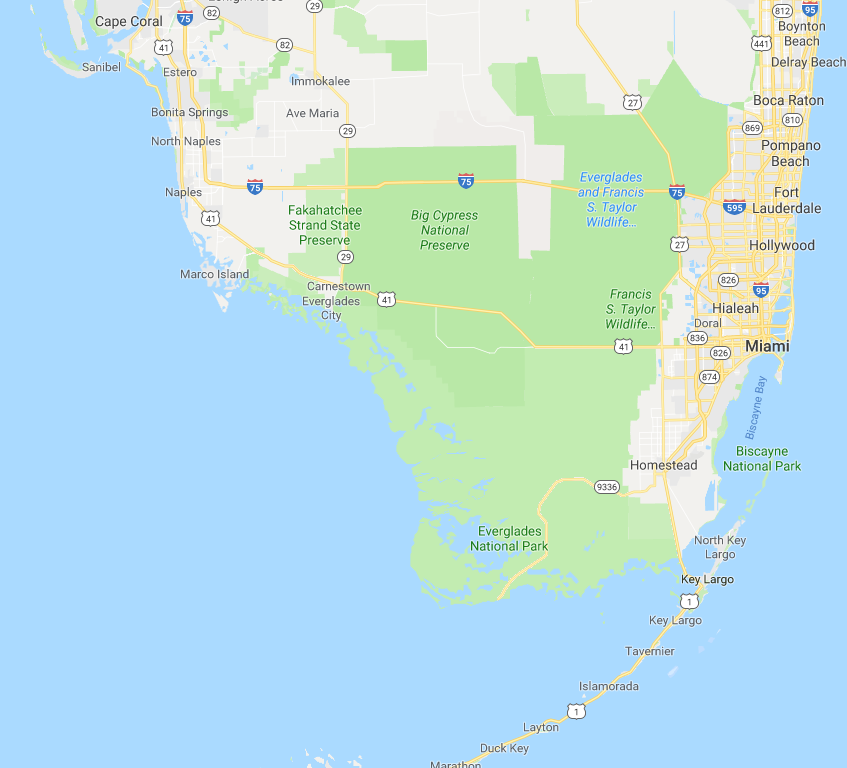
\includegraphics[width=1\linewidth]{images/SouthFloridaPoliticalMap.png} 
    \caption{The Google Maps Political Map allows for quick identification of political boundaries, most notably state or national protected areas.} 
    \vspace{4ex}
  \end{minipage}%%
  \begin{minipage}[b]{0.5\linewidth}
    \centering
    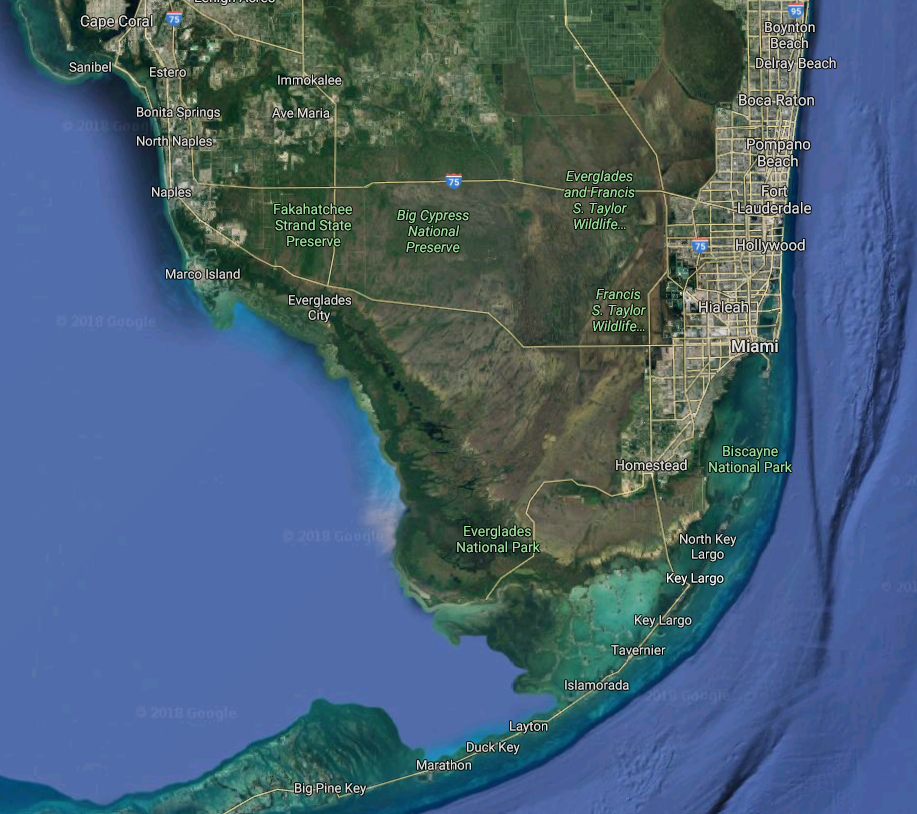
\includegraphics[width=1\linewidth]{images/SouthFloridaSateliteMap.png} 
    \caption{The Google Maps Satellite Map allows for quick identification of natural and artificial reasons why synchrony might be impacted.} 
    \vspace{4ex}
  \end{minipage} 
  \begin{minipage}[b]{0.5\linewidth}
    \centering
    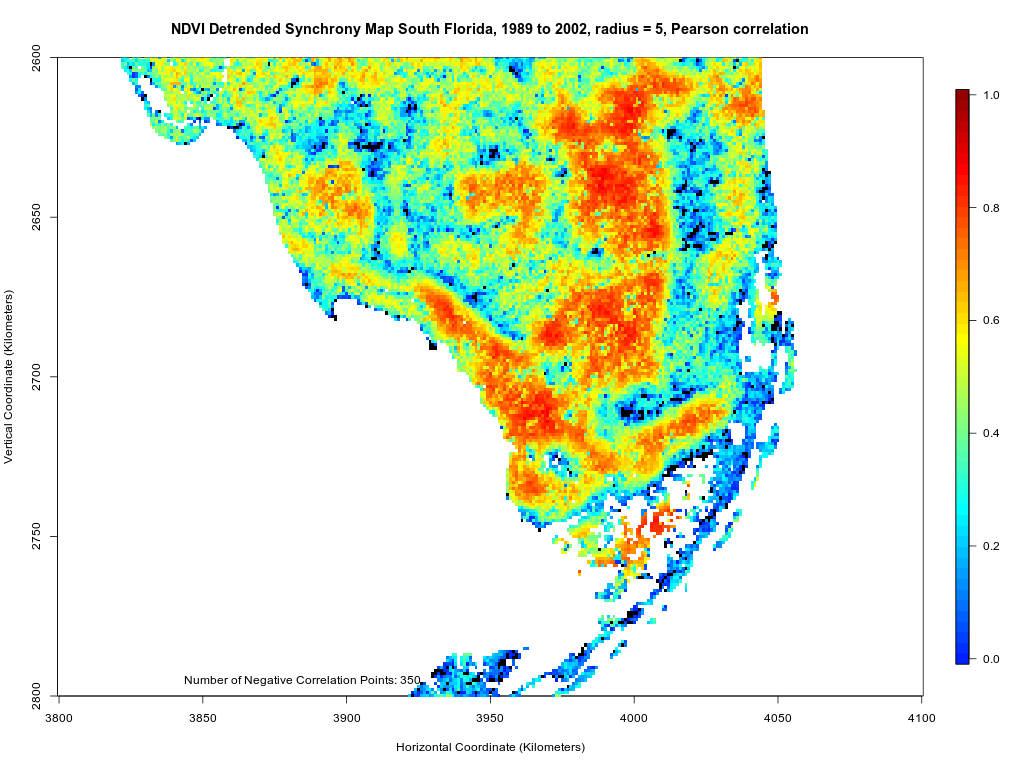
\includegraphics[width=1.1\linewidth]{images/NDVIDetrendedSynchronyMap_SouthFlorida_1989to2002_r5_Pearson.png} 
    \caption{The detrended NDVI synchrony map looked at the time window from 1989 to 2002. It measured the synchrony using the Pearson correlation in a square area with radius of 5 kilometers.} 
    \vspace{4ex}
  \end{minipage}%% 
  \begin{minipage}[b]{0.5\linewidth}
    \centering
    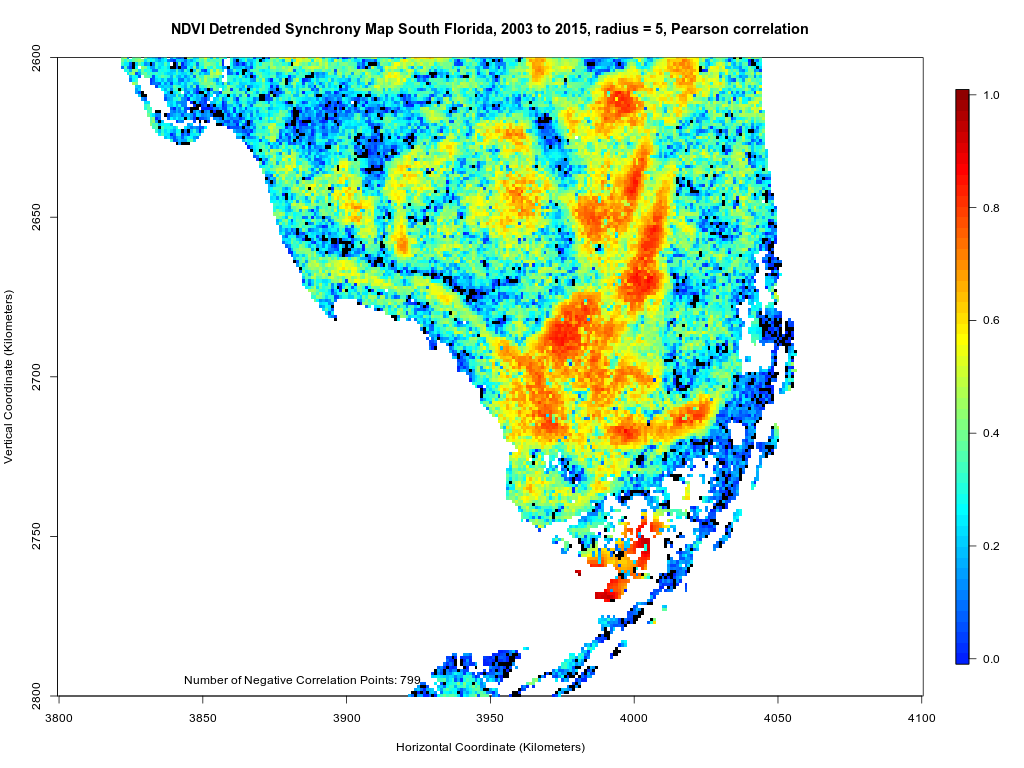
\includegraphics[width=1.1\linewidth]{images/NDVIDetrendedSynchronyMap_SouthFlorida_2003to2015_r5_Pearson.png} 
    \caption{The detrended NDVI synchrony map looked at the time window from 2003 to 2015. It measured the synchrony using the Pearson correlation in a square area with radius of 5 kilometers.} 
    \vspace{4ex}
  \end{minipage} 
\end{figure}
\subsection{Areas of Stable Synchrony}
This section will list areas that remained stable throughout both time windows.
\begin{enumerate}
    \item Miami Metro Area - The entire metro area spans almost the entire eastern coastline from Homestead, Florida in the South until the end of Broward County north of the map. The western boundary of the Miami area is the Everglades. Both windows show a \b{stable and low} synchrony for the entire Miami area, except a marked decrease in the area around the central to north central area.\\
    \item US Highway 41 - US highway 41 cuts a band of \b{stable low synchrony} through the Everglades, especially the eastern half. US highway 41 runs from Naples, Florida on the eastern coast, through the Everglades and connects to Miami on the other side. It's effect is seen most drastically in the 1989 to 2002 window.\\
    \item Southern Everglades National Park - The Everglades as a region has been impacted differently in different areas. The part of the park that remains south of US highway 41 and east of Big Cypress National Preserve shows a \rtext{relatively stable high synchrony area}, although isolated areas like the very southwest part of the park show a decrease.\\
    \item Southern Frances S. Taylor Wildlife Management Area - Parts of this area, mainly in the south and east of the management area, show \r{stable high synchrony}, which cannot be said for the rest of the area.\\
    \item Gap Between the Big Cypress National Preserve and Frances S. Taylor Wildlife Management Area - Looking carefully, there is an area of \b{low synchrony} in the gap between these two protected areas. This gap, while it expands westward towards the Big Cypress National Preserve in the 2003-2015 window, remains relatively stable.
\end{enumerate}
\subsection{Areas of Increasing Synchrony}
This section lists areas that showed an \rtext{increase} of synchrony from the 1989-2002 window to the 2003-2015 window. Very few areas in South Florida show an increase in synchrony.
\begin{enumerate}
    \item Southeastern Everglades National Park - There is a small region of low synchrony that appears to be raised to \rtext{extremely high} synchrony, around state highway 9336. Perhaps the structure of the road was altered to allow for an increase? Or perhaps this region has been a focus of conservation efforts?\\
    \item At the very top center of the 1989-2002 map, there is a small spot of low synchrony. In the 2003-2015 map, it appears to have \rtext{increased substantially}. Google maps shows that region to be farmland.
\end{enumerate}
\subsection{Areas of Decreasing Synchrony}
This section lists areas that showed a \b{decrease} of synchrony from the 1989-2002 window to the 2003-2015 window. The list of decreasing synchronous areas in South Florida is a little larger than the increasing area.
\begin{enumerate}
    \item Western Coast of South Florida - The western coast shows a major \b{decrease} across the board. Google Maps reveals that the region has cities around that area, and it is possible that a recent expansion of that area may be the reason for the decrease.\\
    \item Big Cypress Nation Preserve - This entire region was never a huge source of high synchrony, but almost all of its high areas in the 1989-2002 window show a \b{decrease} in the 2003-2015 regions.\\
    \item Northern Frances S. Taylor Wildlife Management Area - There is a gap of \b{low} synchrony in the wildlife management area in the 2003-2015 map not seen in the 1989-2002 map. Looking closely at the satellite view of Google Maps, there is a manmade canal right in the center of the gap that traces perfectly with the lower synchrony path cut in the high synchrony area.\\
    \item Southern Coast of South Florida - It appears that the southern coast also shows \b{decreases} across the board. Perhaps development or factors impacting the Gulf of Mexico and the Atlantic Sea are impacting the Floridian coastlines.
\end{enumerate}
\subsection{Discussion}
There are many suspected reasons why the synchrony has changed quite dramatically in South Florida.
\begin{enumerate}
    \item Climate Change - The traditional Moran effects fall into this category. Data on yearly rainfall, number of hurricans, and surface temperatures might shed some light on the issue.\\
    \item Local Pollution - I seem to recall that the Everglades is suffering because it serves as the destination for all of the runoff from some major urban centers as well as the upstate farms. Agricultural pollution may be harming the Everglades.\\
    \item Evasive Species - On the same vein, evasive plant species are a major problem in Florida and may be causing some changes in NDVI synchrony (although I'm not sure how to test for this effect....).\\
    \item Increased Urbanization - Florida has has a population explosion, and over 10 million people moved to Florida from 2000 to 2015 (\url{http://worldpopulationreview.com/states/florida-population/}).
\end{enumerate}
%%%%%%%%%%%%%%%%%%%%%%%%%%%%%%%%%%%%%%%%%%%%%%%%
% Geography of Synchrony in the Central Valley
%%%%%%%%%%%%%%%%%%%%%%%%%%%%%%%%%%%%%%%%%%%%%%%%
\section{Geography of Synchrony in Central Valley}
\begin{figure}[ht] 
  \label{CentralValleyMaps} 
  \begin{minipage}[b]{0.5\linewidth}
    \centering
    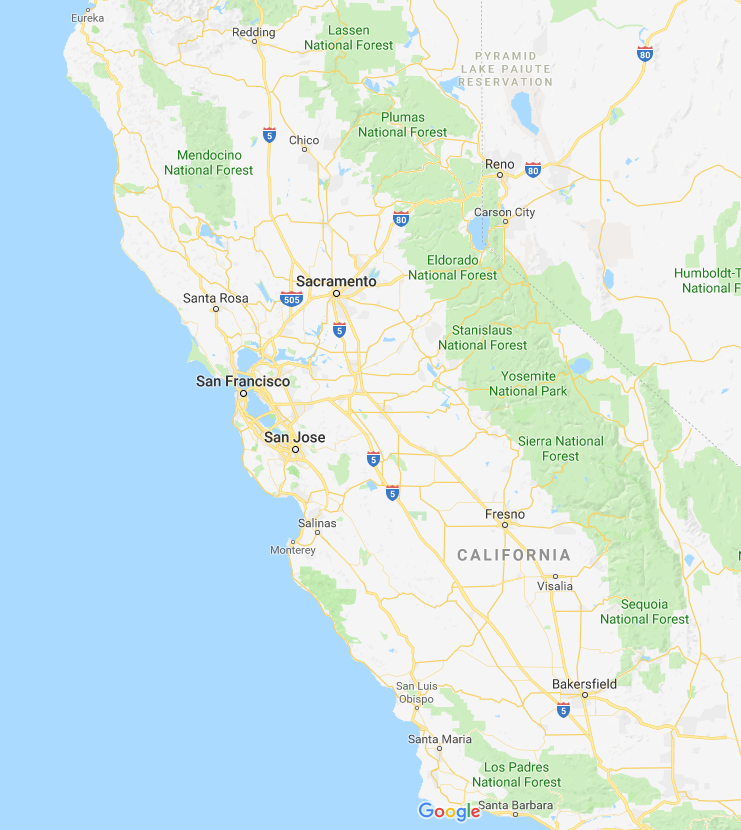
\includegraphics[width=.8\linewidth]{images/CentralValleyPoliticalMap.png} 
    \caption{The Google Maps Political Map allows for quick identification of political boundaries, most notably state or national protected areas.} 
    \vspace{4ex}
  \end{minipage}%%
  \begin{minipage}[b]{0.5\linewidth}
    \centering
    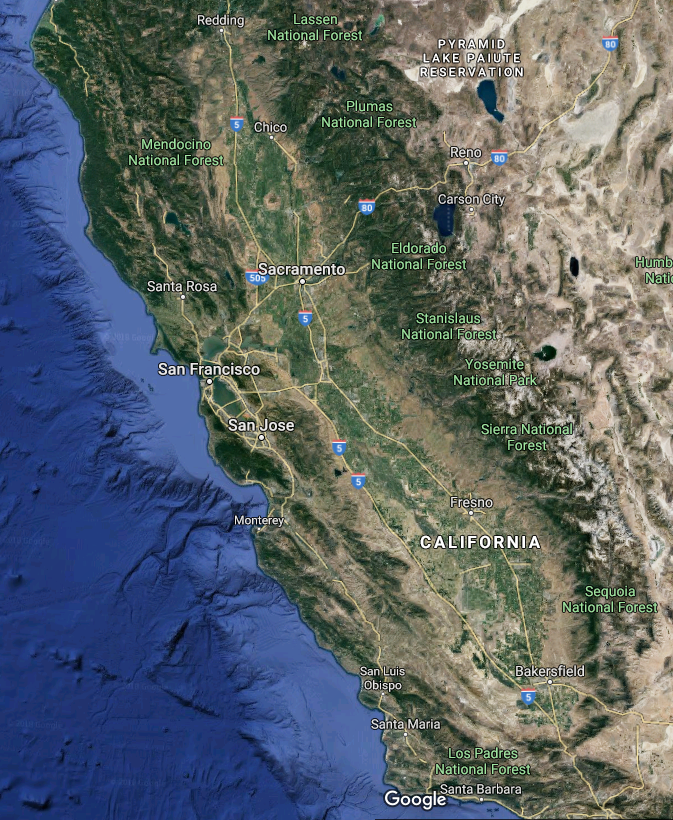
\includegraphics[width=.8\linewidth]{images/CentralValleySatelliteMap.png} 
    \caption{The Google Maps Satellite Map allows for quick identification of natural and artificial reasons why synchrony might be impacted.} 
    \vspace{4ex}
  \end{minipage} 
  \begin{minipage}[b]{0.5\linewidth}
    \centering
    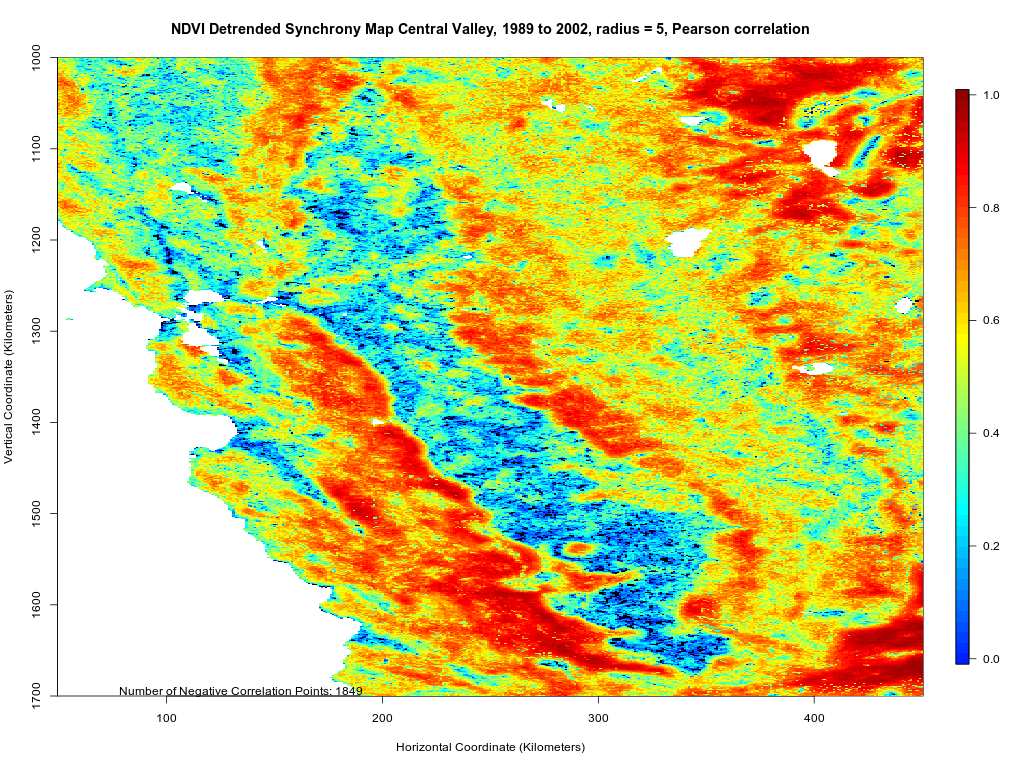
\includegraphics[width=1\linewidth]{images/NDVIDetrendedSynchronyMap_CentralValley_1989to2002_r5_Pearson.png} 
    \caption{The detrended NDVI synchrony map looked at the time window from 1989 to 2002. It measured the synchrony using the Pearson correlation in a square area with radius of 5 kilometers.} 
    \vspace{4ex}
  \end{minipage}%% 
  \begin{minipage}[b]{0.5\linewidth}
    \centering
    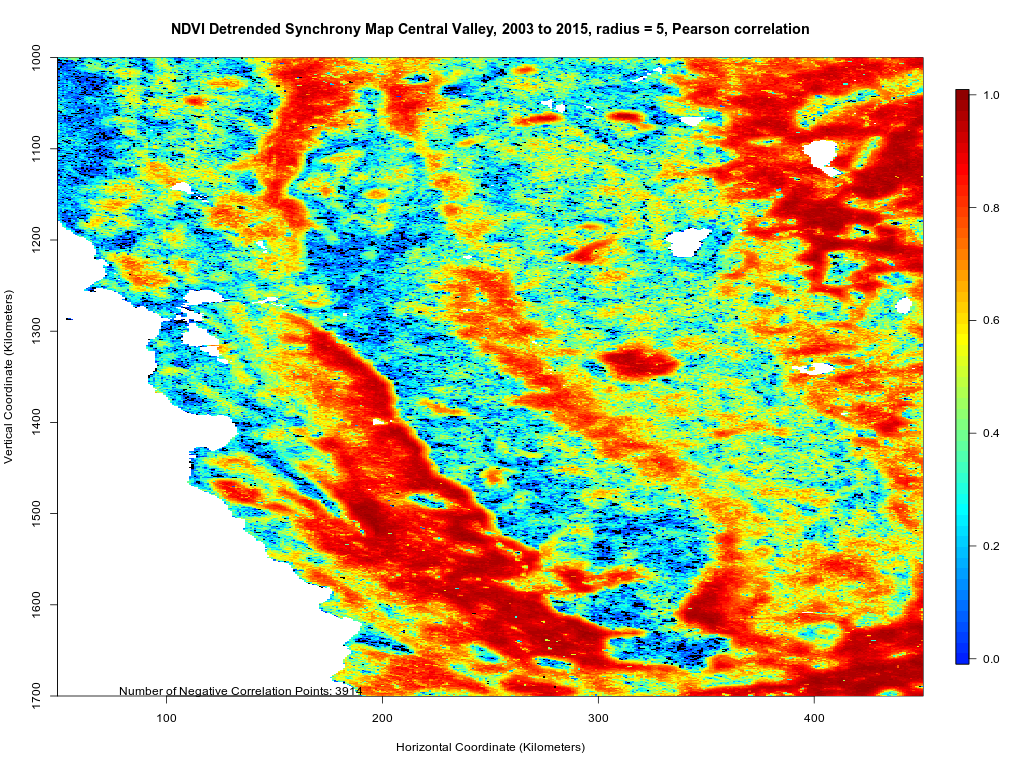
\includegraphics[width=1\linewidth]{images/NDVIDetrendedSynchronyMap_CentralValley_2003to2015_r5_Pearson.png} 
    \caption{The detrended NDVI synchrony map looked at the time window from 2003 to 2015. It measured the synchrony using the Pearson correlation in a square area with radius of 5 kilometers.} 
    \vspace{4ex}
  \end{minipage} 
\end{figure}
%%%%%%%%%%%%%%%%%%%%%%%%%%%%%%%%%%%%%%%%%%%%%%%%
% Geography of Synchrony in Mississippi
%%%%%%%%%%%%%%%%%%%%%%%%%%%%%%%%%%%%%%%%%%%%%%%%
\section{Geography of Synchrony in Mississippi River Delta}
\begin{figure}[ht] 
  \label{CentralValleyMaps} 
  \begin{minipage}[b]{0.5\linewidth}
    \centering
    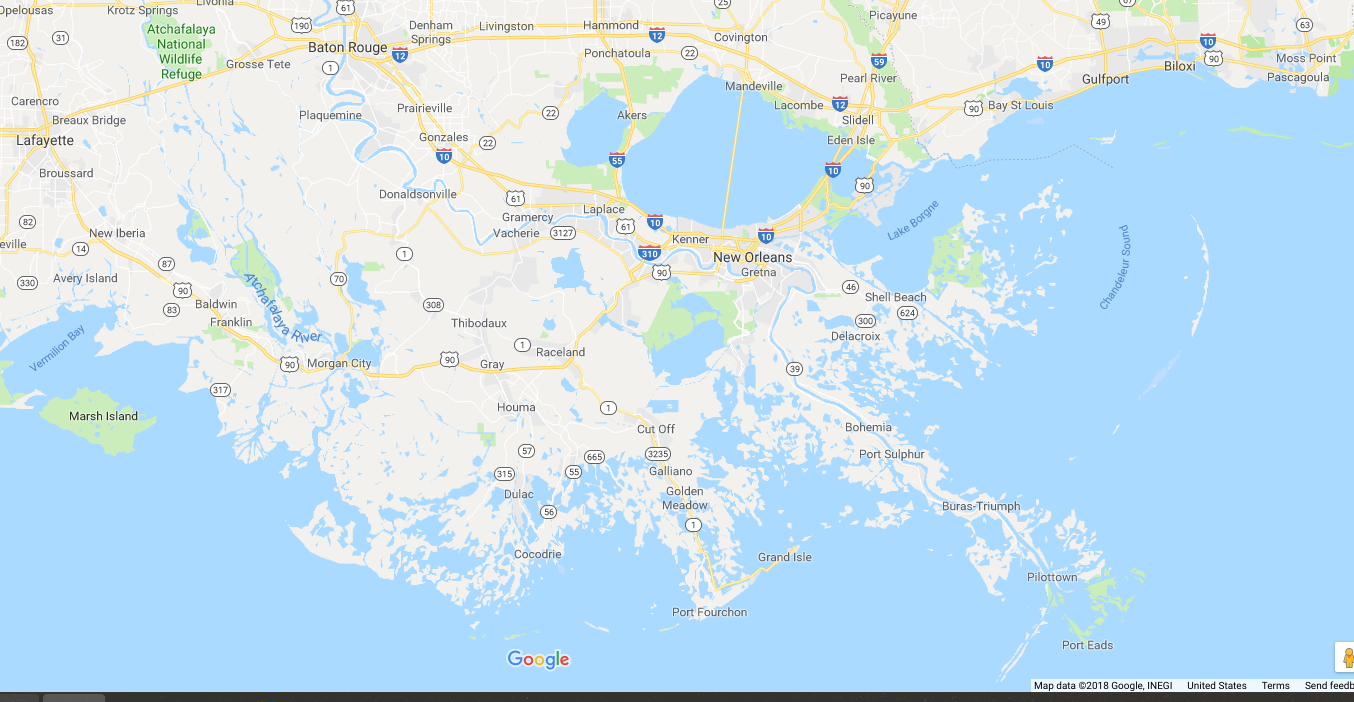
\includegraphics[width=.8\linewidth]{images/MississippiDeltaPolitical_Google_2018.png}
    \caption{The Google Maps Political Map allows for quick identification of political boundaries, most notably state or national protected areas.} 
    \vspace{4ex}
  \end{minipage}%%
  \begin{minipage}[b]{0.5\linewidth}
    \centering
    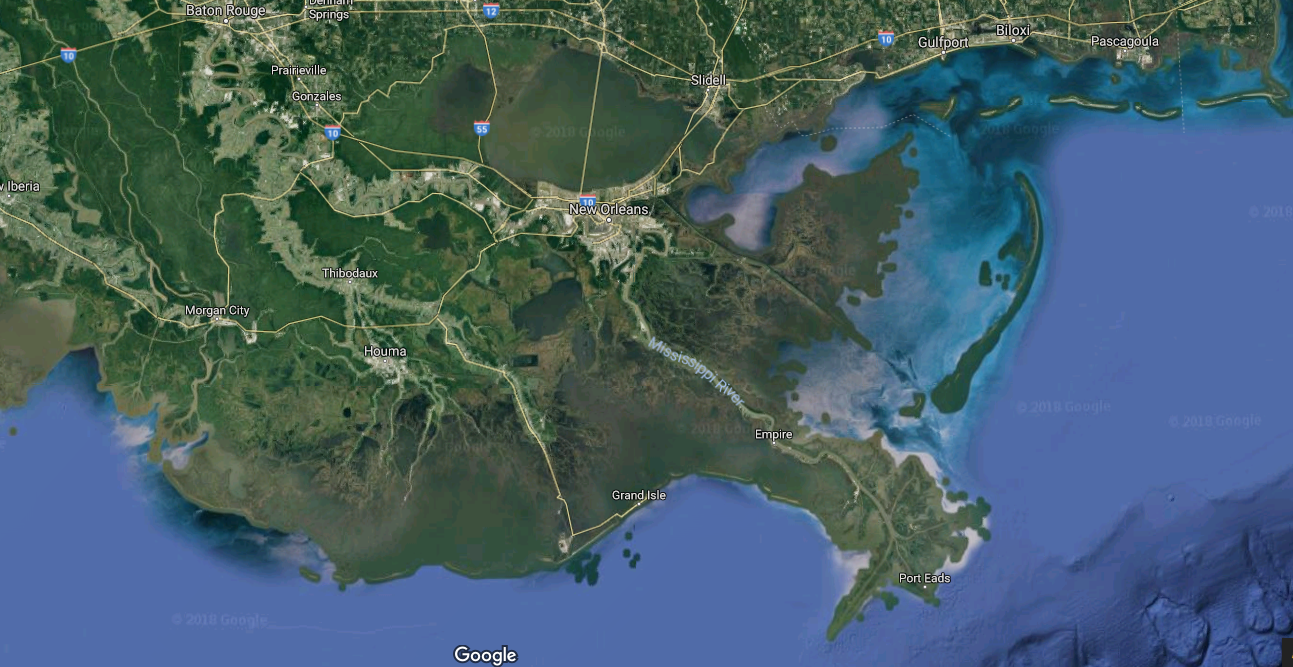
\includegraphics[width=.8\linewidth]{images/MississippiDeltaGoogleSatPic_2018.png} 
    \caption{The Google Maps Satellite Map allows for quick identification of natural and artificial reasons why synchrony might be impacted.} 
    \vspace{4ex}
  \end{minipage} 
  \begin{minipage}[b]{0.5\linewidth}
    \centering
    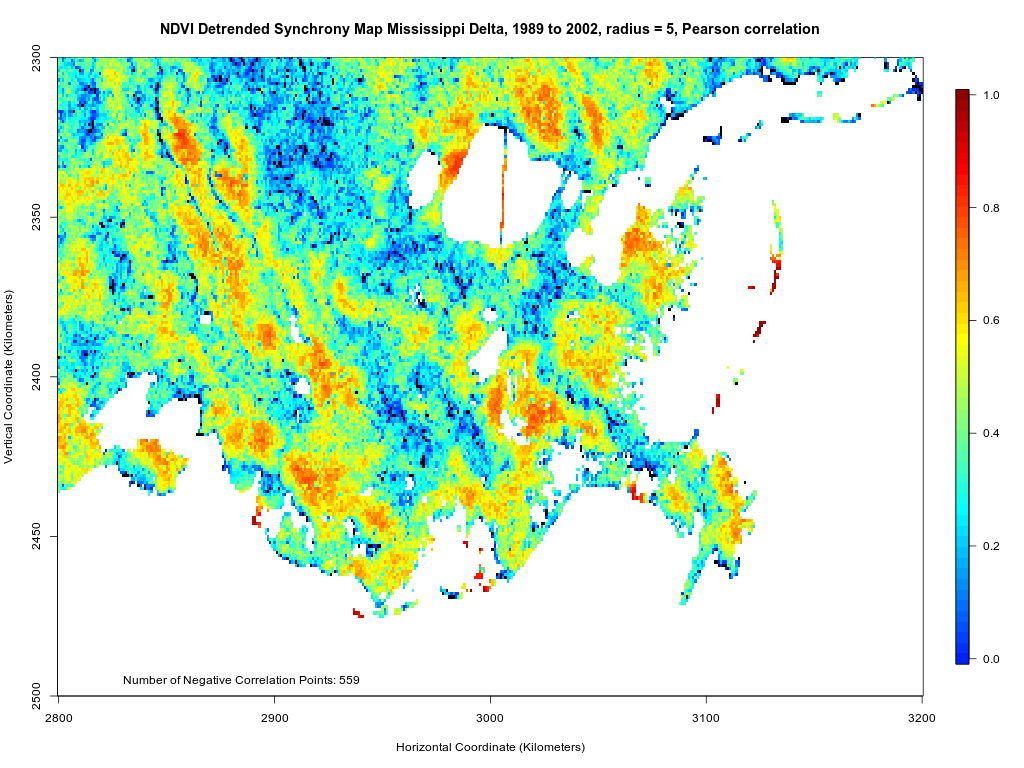
\includegraphics[width=1\linewidth]{images/NDVIDetrendedSynchronyMap_MississippiDelta_1989to2002_r5_Pearson.png} 
    \caption{The detrended NDVI synchrony map looked at the time window from 1989 to 2002. It measured the synchrony using the Pearson correlation in a square area with radius of 5 kilometers.} 
    \vspace{4ex}
  \end{minipage}%% 
  \begin{minipage}[b]{0.5\linewidth}
    \centering
    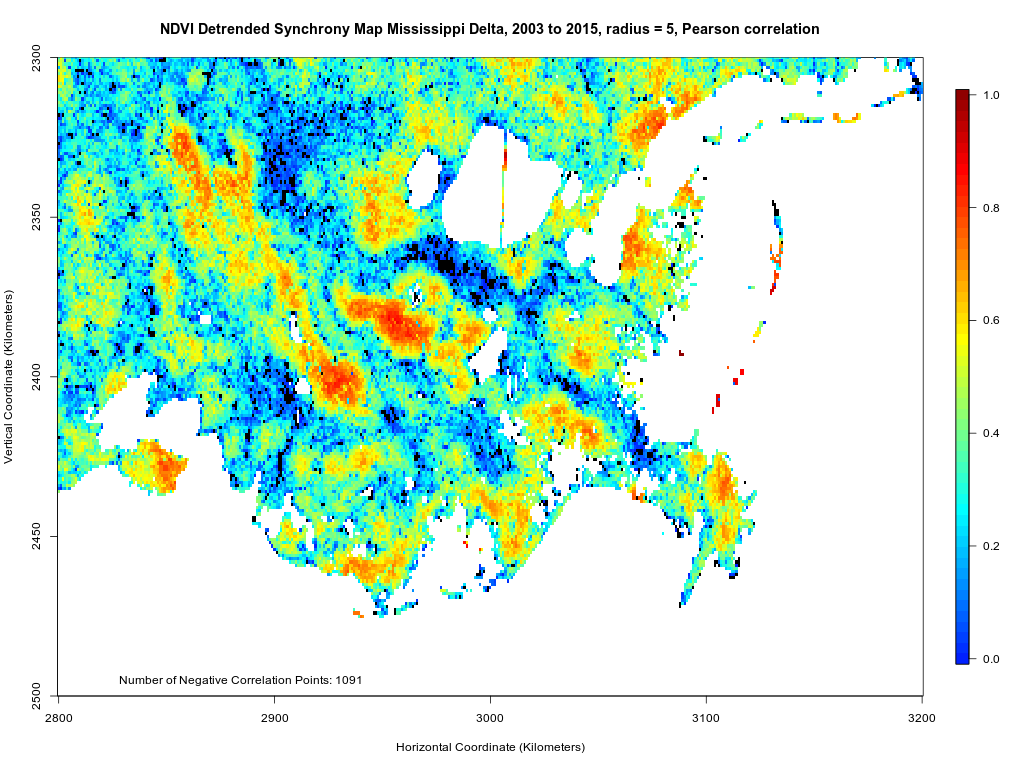
\includegraphics[width=1\linewidth]{images/NDVIDetrendedSynchronyMap_MississippiDelta_2003to2015_r5_Pearson.png} 
    \caption{The detrended NDVI synchrony map looked at the time window from 2003 to 2015. It measured the synchrony using the Pearson correlation in a square area with radius of 5 kilometers.} 
    \vspace{4ex}
  \end{minipage} 
\end{figure}
%%%%%%%%%%%%%%%%%%%%%%%%%%%%%%%%%%%%%%%%%%%%%%%%
% Conclusions
%%%%%%%%%%%%%%%%%%%%%%%%%%%%%%%%%%%%%%%%%%%%%%%%
\section{Conclusion}
\end{document}
